\documentclass[tikz,border=2pt,png]{standalone}
\usepackage{tkz-euclide}
\begin{document}
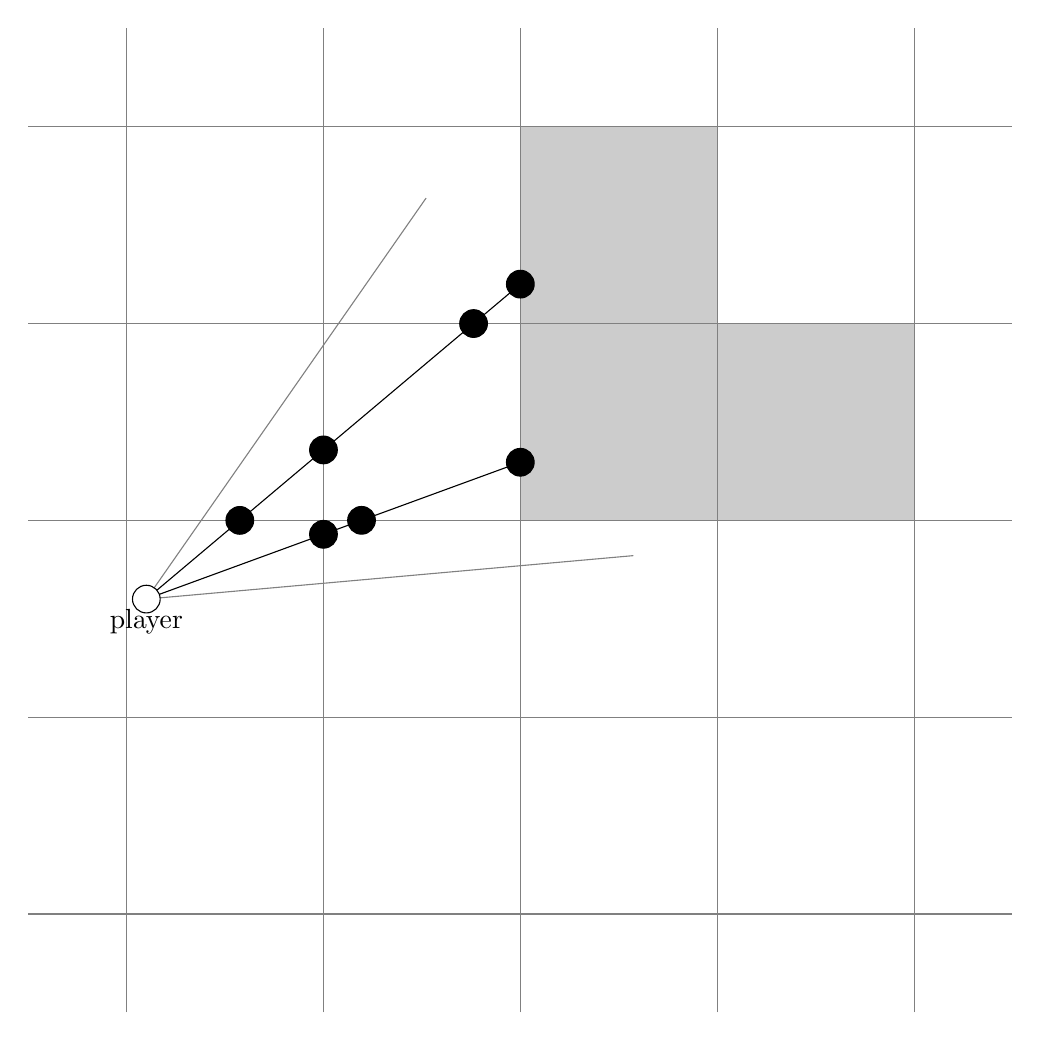
\begin{tikzpicture}[scale=2.5]


\coordinate(player) at (2.1,3.6) {};
\coordinate(intercept) at (4,5.2) {};






\fill[black!20!white, draw=black] (4,5) rectangle (5,6);
\fill[black!20!white, draw=black] (4,4) rectangle (5,5);
\fill[black!20!white, draw=black] (5,4) rectangle (6,5);

%grid
% vertical lines
\draw[draw=gray] (2,1.5) -- (2,6.5) ;
\draw[draw=gray] (3,1.5) -- (3,6.5) ;
\draw[draw=gray] (4,1.5) -- (4,6.5) ;
\draw[draw=gray] (5,1.5) -- (5,6.5) ;
\draw[draw=gray] (6,1.5) -- (6,6.5) ;

% horizontal lines
\draw[draw=gray] (1.5,2) -- (6.5,2) ;
\draw[draw=gray] (1.5,3) -- (6.5,3) ;
\draw[draw=gray] (1.5,4) -- (6.5,4) ;
\draw[draw=gray] (1.5,5) -- (6.5,5) ;
\draw[draw=gray] (1.5,6) -- (6.5,6) ;
%\draw[] 

%FOV
\coordinate[](left_edge) at ($(player)!1!15:(intercept)$);
\coordinate[](right_edge) at ($(player)!1!325:(intercept)$);
\draw[draw=gray] (player) -> (left_edge) ;
\draw[draw=gray] (player) -> (right_edge) ;

\draw[draw=black] (player) -- (intercept) ;

\fill[draw=black] (intercept) circle (2pt);

\draw(player)node[below]{player};

% check points for first intercept
\coordinate(line1_p1) at (0,4) {};
\coordinate(line1_p2) at (9,4) {};
\coordinate (check1) at (intersection of player--intercept and line1_p1--line1_p2);
\fill[draw=black] (check1) circle (2pt);

\coordinate(line2_p1) at (0,5) {};
\coordinate(line2_p2) at (9,5) {};
\coordinate (check2) at (intersection of player--intercept and line2_p1--line2_p2);
\fill[draw=black] (check2) circle (2pt);

%vertical intercelpt
\coordinate(line3_p1) at (3,0) {};
\coordinate(line3_p2) at (3,9) {};
\coordinate (check3) at (intersection of player--intercept and line3_p1--line3_p2);
\fill[draw=black] (check3) circle (2pt);



%intercept 2
\coordinate[](missed_intercept) at ($(player)!1!340:(intercept)$);


\coordinate(i2_line1_p1) at (0,4) {};
\coordinate(i2_line1_p2) at (9,4) {};
\coordinate (i2_check1) at (intersection of player--missed_intercept and i2_line1_p1--i2_line1_p2);
\fill[draw=black] (i2_check1) circle (2pt);

%vertical intercelpt
\coordinate(i2_line2_p1) at (4,0) {};
\coordinate(i2_line2_p2) at (4,9) {};
\coordinate (i2_check2) at (intersection of player--missed_intercept and i2_line2_p1--i2_line2_p2);
\fill[draw=black] (i2_check2) circle (2pt);


\coordinate(i2_line3_p1) at (3,0) {};
\coordinate(i2_line3_p2) at (3,9) {};
\coordinate (i2_check3) at (intersection of player--missed_intercept and i2_line3_p1--i2_line3_p2);
\fill[draw=black] (i2_check3) circle (2pt);
\draw[draw=black] (player) -- (i2_check2) ;

\fill[draw=black, fill=white] (player) circle (2pt);

\end{tikzpicture}
\end{document}
